\documentclass[a4paper,12pt]{article}
\usepackage{setspace}
\usepackage[english]{babel}
\usepackage[utf8]{inputenc}
\usepackage[margin=2.54cm]{geometry}
\usepackage{pdfpages}
\usepackage[utf8]{inputenc}
\usepackage[catalan]{babel}
\usepackage{graphicx,subcaption}
\usepackage{graphics}
\usepackage{lscape}
\usepackage{pdflscape}
\usepackage{float}
\usepackage{textcomp}
\usepackage{amsmath}
\usepackage{hyperref}
\usepackage{fancyvrb}
\usepackage{parskip}
\usepackage{changepage}
\usepackage{enumitem}
\usepackage{tcolorbox}
\usepackage[all]{hypcap}
\usepackage{xcolor}
\usepackage{listings}
\definecolor{green}{HTML}{228B22}
\definecolor{orange}{HTML}{FFA528}
\lstset{
    frame=tb, % draw a frame at the top and bottom of the code block
    tabsize=4, % tab space width
    showstringspaces=false, % don't mark spaces in strings
    numbers=left, % display line numbers on the left
    commentstyle=\color{green}, % comment color
    keywordstyle=\color{blue}, % keyword color
    stringstyle=\color{red}, % string color
    breaklines=true,
    numbers=left,
    xleftmargin=2em,
    framexleftmargin=1.5em,
    %postbreak=\mbox{\textcolor{red}{$\hookrightarrow$}\space},
}

\hypersetup{
    colorlinks,
    citecolor=black,
    filecolor=black,
    linkcolor=black,
    urlcolor=black
}
\title{
	\begin{center}
	\vspace{3cm}
	
\includegraphics[width=11cm, height=3cm]{images/logo_eps.png}
	\end{center}
	\begin{center}
	\line(1,0){340}
	\end{center}		
	SOFTWARE AND HARDWARE VALIDATION SYSTEMS\\
	\vspace{2mm}
	\Large Practical case 1: Verification of programs with Hoare logic and symbolic execution\\
	\line(1,0){340}
	\vspace{1.5cm}
	}

\author{Joel Aumedes Serrano - 48051307Y \\ Marc Cervera Rosell - 47980320C \vspace{1cm}}


\date{Academic course 2021 - 22\vspace{0.5cm} \\Bachelor's degree in computer engineering}
\onehalfspacing

\begin{document}
	\begin{titlepage}
		\maketitle
		\thispagestyle{empty}
	\end{titlepage}
	\cleardoublepage
	\newpage

\tableofcontents
\listoffigures
\thispagestyle{empty}

\newpage

\section{Exercise 1}
\begin{figure}[H]
    \centering
	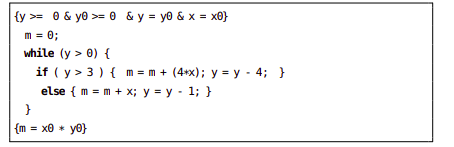
\includegraphics[scale = 1.0]{images/Screenshot from 2022-03-30 16-23-46.png}
	\caption{Exercise 1 code}
	\label{fig:code1}
\end{figure}
\justify{\textbf{\textit{Statement:}\\
Considering the breathtaking algorithm (see Figure~\ref{fig:code1}) for the multiplication of two integer numbers you must:\\
1. Obtain an appropiate invariant for the loop and explain it\\
2. Perform the verification of the partial correctness of the algorithm.}}
\pagenumbering{arabic}

\newpage

\section{Exercise 2}
\begin{figure}[H]
    \centering
	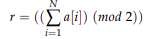
\includegraphics[scale = 1.0]{images/formula.png}
	\caption{Exercise 2 formula}
	\label{fig:formula1}
\end{figure}
\begin{figure}[H]
    \centering
	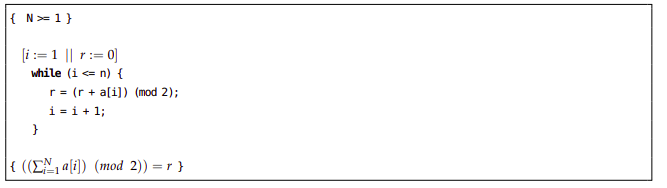
\includegraphics[scale = 0.70]{images/codi.png}
	\caption{Exercise 2 code}
	\label{fig:code2}
\end{figure}
\justify{\textbf{\textit{Statement:\\}
Verify the algorithm of the Figure~\ref{fig:code2} for computing the parity of the sum of the elements of an array a[N] with N \textbf{$\geq 0$} and storing it in the result variable r. You must:\\
1. Obtain an appropriate invariant for the loop and explain it.\\
2. Perform the verification of the partial correctness of the algorithm.}}



\end{document}
